\documentclass[hyperref={pdfpagelabels=false}]{beamer}

\usepackage{xeCJK}
\setCJKmainfont[AutoFakeSlant=0.25]{Noto Sans Mono CJK SC}
\setCJKsansfont[AutoFakeSlant=0.25]{Noto Sans Mono CJK SC}
\setCJKmonofont[AutoFakeSlant=0.25]{Noto Sans Mono CJK SC}

\usepackage{python}
\usepackage{lmodern}
\usepackage{url}
\usepackage{hyperref}
\usepackage{listings}
\usepackage{xcolor}
\hypersetup{
	colorlinks=true,
	linkcolor=blue,
	filecolor=blue,
	citecolor = black,      
	urlcolor=blue,
}

\definecolor{codegreen}{rgb}{0,0.6,0}
\definecolor{codegray}{rgb}{0.5,0.5,0.5}
\definecolor{codepurple}{rgb}{0.58,0,0.82}
\definecolor{backcolour}{rgb}{0.95,0.95,0.92}

\lstdefinestyle{mystyle}{
    backgroundcolor=\color{backcolour},   
    commentstyle=\color{codegreen},
    keywordstyle=\color{magenta},
    numberstyle=\tiny\color{codegray},
    stringstyle=\color{codepurple},
    basicstyle=\ttfamily\footnotesize,
    breakatwhitespace=false,         
    breaklines=true,                 
    captionpos=b,                    
    keepspaces=true,                                    
    numbersep=5pt,                  
    showspaces=false,                
    showstringspaces=false,
    showtabs=false,                  
    tabsize=2
}

\lstset{style=mystyle}

\usetheme{Madrid}
\usecolortheme{dolphin}
\title{软件开发过程中平台兼容性分析}  
\subtitle{Windows和linux之间的兼容性开发}
\author{叶茂青} 
\date{\today} 
\begin{document}
\begin{frame}
\titlepage
\end{frame} 

\begin{frame}
	\frametitle{总览}
	\tableofcontents
\end{frame} 

\section{什么是兼容}
\begin{frame}
	\tableofcontents[currentsection]
\end{frame} 

\begin{frame}
	\frametitle{什么是兼容}
	\begin{itemize}
		\item 二进制兼容:对于一个可执行文件,不需要做任何修改就可以直接运行
		\item 源码兼容:在新的系统上,不需要更改源码,只需要重新编译或利用解释器即可运行
		\item 向前兼容:新程序能接受老程序的输入
		\item 向后兼容:老程序能接受新程序的输入
	\end{itemize}
\end{frame}

\section{常见的Windows和Linux之间的行为差异}
\begin{frame}
	\tableofcontents[currentsection]
\end{frame}

\begin{frame}
	\frametitle{文件分隔符}
	\begin{columns}
		\begin{column}{.5\linewidth}
			\lstinputlisting[language=python,basicstyle=\tiny]{./code/false1.py}
		\end{column}
	
		\begin{column}{.5\linewidth}
			\begin{itemize}
				\item 由于DOS系统中斜杆被表示为命令行参数
				\item Windows使用\texttt{\textbackslash}作为文件的分隔符
				\item 而Linux使用\texttt{/}作为文件分隔符
			\end{itemize}
		\end{column}
	\end{columns}
\end{frame}

\begin{frame}
	\frametitle{文件分隔符}
	\begin{columns}
		\begin{column}{.5\linewidth}
			\lstinputlisting[language=python,basicstyle=\tiny]{./code/true1.py}
		\end{column}
	
		\begin{column}{.5\linewidth}
			解决方案:
			\begin{itemize}
				\item 统一用\texttt{/}
				\item 交给os库处理
			\end{itemize}
		\end{column}
	\end{columns}
\end{frame}

\begin{frame}
	\frametitle{换行符}
	\begin{columns}
		\begin{column}{.5\linewidth}
			\lstinputlisting[language=python,basicstyle=\tiny]{./code/3.py}
			\begin{figure}
				\centering
				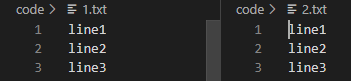
\includegraphics[width=\textwidth]{./figure/1.png}
			\end{figure}
		\end{column}
		\pause
		\begin{column}{.5\linewidth}
			\begin{figure}
				\centering
				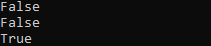
\includegraphics[width=\textwidth]{./figure/2.png}
			\end{figure}
		\end{column}
	\end{columns}
\end{frame}

\begin{frame}
	\frametitle{换行符}
	Windows采用CRLF为换行符,而Linux采用LF为换行符,解决方案:
	\begin{itemize}
		\item 用二进制读写
		\item 在写文件时设定换行符
	\end{itemize}
	\begin{figure}
		\centering
		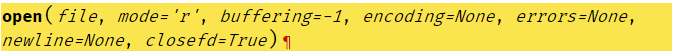
\includegraphics[width=\textwidth]{./figure/3.png}
	\end{figure}
\end{frame}

\begin{frame}
	\frametitle{多进程}
	\begin{columns}
		\begin{column}{.5\linewidth}
			\lstinputlisting[language=python,basicstyle=\tiny]{./code/false2.py}
		\end{column}
	
		\begin{column}{.5\linewidth}
		Linux中由于创建新进程会使用fork(),子进程可以直接获取父进程中的变量
		\end{column}
	\end{columns}
\end{frame}

\begin{frame}
	\frametitle{多进程}
	\begin{columns}
		\begin{column}{.5\linewidth}
			\lstinputlisting[language=python,basicstyle=\tiny]{./code/true2.py}
		\end{column}
	
		\begin{column}{.5\linewidth}
			在Windows中应该显式的进行传递或使用共享内存
		\end{column}
	\end{columns}
\end{frame}

\begin{frame}
	\frametitle{参考文献}
	\href{https://stackoverflow.com/questions/6596617/python-multiprocess-diff-between-windows-and-linux}{multiprocessing - Python Multiprocess diff between Windows and Linux - Stack Overflow}\\
	~\\
	\href{https://docs.microsoft.com/zh-cn/archive/blogs/larryosterman/why-is-the-dos-path-character}{Why is the DOS path character ""?}\\
	~\\
	\href{https://devblogs.microsoft.com/oldnewthing/20040318-00/?p=40193}{Why is the line terminator CR+LF?}\\
	~\\
	\href{https://docs.python.org/2/library/multiprocessing.html}{python multiprocessing guidelines}
\end{frame}

\begin{frame}{}
	\centering \Huge
	\emph{Thank You!}
\end{frame} 

\end{document}

